\section{Exact-model check and synthetic intervention}
\label{sec:synthetic}

\paragraph{Experiment 1: the exact model.}
The closed forms of Theorem~\ref{thm:serial} were checked against a full
$(2+M)$-parameter integration of the flow over $525$ initialization--width--margin
cases and a Gaussian initialization sweep (Section~\ref{sec:theorem},
Appendix~\ref{app:verification}); every bound holds in every case. This is a
check of the algebra. The question the rest of the paper asks is whether the
mechanism survives when the cues are noisy, the routing is learned and the
head is nonlinear.

\paragraph{Experiment 2: design.}
Pixels carry i.i.d.\ labels $y_p\in\{-1,+1\}$ on $16\times16$ images with
$S=256$ spectral channels, so the spectral cue cannot be denoised by
averaging neighbours. The spectral cue is $\alpha y_pu$ in the pixel's own
spectrum, buried in isotropic noise of unit variance, with $u$ a fixed unit
direction the encoder must discover. The contextual cue places $y_p$ in
each of the eight neighbours of $p$, along eight fixed orthogonal
directions $v_1,\dots,v_8\perp u$ of amplitude $\beta=5$ with context noise
$\tau\eta$: the information about $y_p$ sits only in the neighbourhood,
because $p$'s own $v$-coordinates carry its neighbours' labels. Equal
information: $\alpha=1.645$ gives an oracle spectral accuracy of $0.95$,
and $\tau=1.70$ is calibrated so that the oracle contextual accuracy (a
linear discriminant on the $3\times3$ window of the eight projections) is
$0.950$; both values are recorded before any training run
(Appendix~\ref{app:exp2}). Readiness: through a random encoder
$W\in\R^{12\times256}$ the same discriminant reads the contextual cue at
$0.905$--$0.914$ and the spectral cue at $0.608$--$0.653$ (three seeds),
because the random projection preserves the signal-to-noise ratio of a
cue whose noise shares its direction and attenuates by about $\sqrt{K/S}$
one whose noise is isotropic. This is the nonlinear analogue of
$(a_0\ \text{small},\ v_0=O(1))$: the contextual cue is initially
accessible to a trained readout; the spectral cue is not. The model is the
linear encoder followed by a ReLU convolutional head
($3\times3$ convolution to width $M$, ReLU, $3\times3$ convolution to one
logit, circular padding), trained by full-batch gradient descent on
$256$ images ($65{,}536$ pixels) with one learning rate $\eta=10^{-3}$ for
every parameter, chosen as the largest rate with a monotone loss at the
widest head. Runs are compared at the first step with training loss below
$L^\ast=0.30$, with further snapshots at $0.6,0.5,0.4,0.2,0.15,0.10$.

\paragraph{Arms and measures.}
Standard parameterization at widths $M\in\{2,4,8,32,128,512,2048\}$; a
normalized readout ($M^{-1/2}\gamma$ with $\gamma=O(1)$ and the same
function at initialization, the control of Theorem~\ref{thm:serial}(c),
which under plain gradient descent equals a readout trained at rate $1/M$);
training with an uninformative context (the same cue carrying an
independent label: the proposed cause removed) at $M\in\{2,8,128,512\}$;
a readout learning-rate multiplier and, following the design review, a
whole-head multiplier $\kappa\in\{1,1/16,1/256\}$ at $M=32$, which in the
theorem gives the bound $1/(1+\kappa Mv_0^2)$; and a frozen encoder. Three
seeds each. At every snapshot we record the encoder's linear accessibility
of the spectral cue (a discriminant fitted on independent spectral-only
data and evaluated on a disjoint set, reported as the gain over its initial
value $0.647$), the exact population counterpart
$h_u(W)=\|P_{\mathrm{row}(W)}u\|^2$ (the optimal probe has accuracy
$\Phi(\alpha\sqrt{h_u})$; $h_u=0.055$ at initialization), the encoder's
displacement, and accuracies on paired test sets that share labels and
noise and differ only in the assigned context: iid, reversed,
context-random, spectral-only, context-only.

\paragraph{Results: suppression.}
At $L^\ast$ every jointly trained model with an informative context leaves
the encoder's spectral accessibility near its initial value: the probe gain
is $0.04$ at $M=2$ and $0.002$ at $M=2048$ (means over three seeds; $h_u$
$0.09\to0.05$ against $0.055$ at initialization), accuracy under reversal
is $0.12$--$0.13$, and accuracy with an uninformative context is at chance
($0.50$). The same model trained with an uninformative context aligns its
encoder before reaching the same loss (probe gain $0.25$--$0.30$; $h_u$
$0.56$--$0.86$) and survives reversal ($0.88$--$0.90$). A frozen encoder
gives reversal accuracy $0.12$--$0.14$ (Table~\ref{tab:exp2_star}).

\paragraph{Results: the registered predictions.}
We report P1--P5 as registered (Appendix~\ref{app:exp2}). P1 fails: the
width trend in encoder alignment and reversal accuracy is monotone in two
seeds but not the third, and its magnitude is negligible, because $L^\ast$
lies in a regime where the context fits before any spectral adaptation at
every width, including $M=2$. P2 fails as stated (the normalized readout
also shows a small trend in two seeds). P3 fails its literal cutoff on the
encoder's energy fraction while its substance holds: with the cause removed
the encoder exposes the cue at every width (probe $0.89$--$0.94$), the
energy fraction merely spreading over more head directions as $M$ grows.
P4 holds for spectral learning (alignment and probe decrease with the
readout multiplier in every seed) and fails for reversal accuracy, which
rises by $0.02$. P5 holds. A flat curve in a saturated regime does not
falsify competition; it shows that the registered threshold could not
resolve it.

\paragraph{Results: where the width and speed dependence appears.}
At the labelled secondary threshold $0.15$, just above the population
optimum of the contextual cue alone, spectral learning decreases with
width in every seed (probe gain $0.22$ at $M=2$, $0.12$ at $M=8$, $0.06$ at
$M=128$, $0.03$ at $M=2048$; Spearman $-0.86$, $-0.96$, $-0.86$), and the
normalized readout is less suppressed at large width ($0.10$ at $M=2048$
against $0.03$; Table~\ref{tab:exp2_015}). The whole-head multiplier moves
the same quantity at $L^\ast$ itself: probe gain $0.03$, $0.11$, $0.22$ and
$h_u$ $0.08$, $0.18$, $0.48$ for $\kappa=1$, $1/16$, $1/256$ (seed 0;
Table~\ref{tab:exp2_kappa}), in the direction of the theorem's bound
$1/(1+\kappa Mv_0^2)$; at $\kappa\le1/4096$ the head is too slow to reach
$L^\ast$ within the step budget, and the encoder ends with $h_u=0.70$.
The readout-only multiplier acts in the same direction but weakly
(Table~\ref{tab:exp2_lrmult}).

\paragraph{Results: reliance does not follow speed.}
Accuracy under reversal at $L^\ast$ stays between $0.11$ and $0.21$ across
every width, every $\kappa$ including the extension, the normalized readout
and the readout multiplier, and accuracy with an uninformative context
stays at chance; only training without an informative context removes the
reliance. The encoder can be made to expose the cue almost fully ($h_u$
$0.70$, probe $0.91$) while the head still predicts from context. In the
theorem's terms the fitted models sit in the regime $2a(T_m)<m$: the
contextual pathway's speed relative to the encoder controls how much of
the spectral cue the encoder learns before the fit is reached; the head's
gain for the large-amplitude contextual cue, which slowing the whole head
leaves unchanged, controls which cue the fitted head uses. The probe is a
linear readout on the frozen encoder, so it measures what readout
retraining without the shortcut can recover \citep{kirichenko2023dfr}: a
fast wide head leaves $0.65$--$0.75$ recoverable spectral accuracy, a slow
head, a small width, a normalized readout at large width or an
uninformative context leave $0.87$--$0.94$.

\paragraph{Amendments.}
Widths $2$ and $4$, the fractional readout multipliers and the whole-head
arm were added after a one-seed pilot and the design review, before the
corresponding runs; the $\kappa$ bracket was extended downward for the
reversal outcome after the seed-0 pilot (Appendix~\ref{app:exp2}). The
original five-width predictions are reported above as registered.

\begin{figure}[t]
\centering
\IfFileExists{figures/fig3_exp2.pdf}{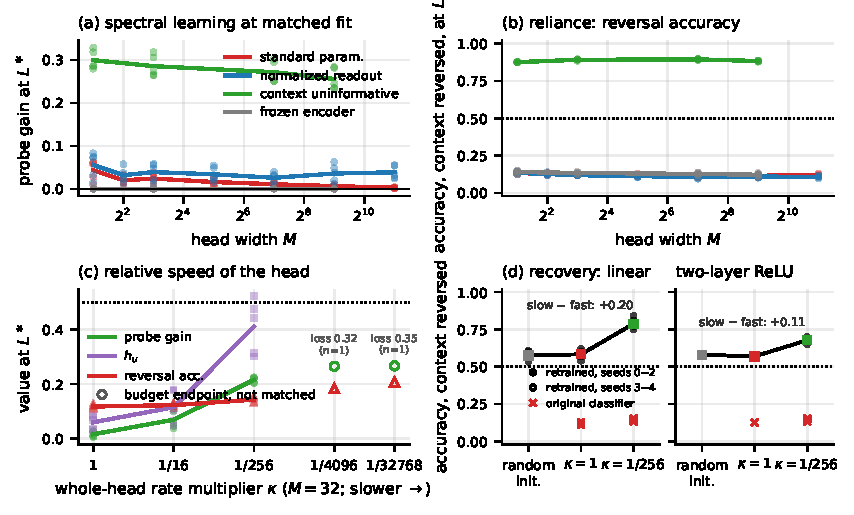
\includegraphics[width=\linewidth]{figures/fig3_exp2.pdf}}{\fbox{\rule{0pt}{2.0in}\rule{0.97\linewidth}{0pt}}}
\caption{Experiment 2 at matched fit $L^\ast=0.30$ (three seeds; points are
seeds, lines are means). (a) Spectral probe gain over initialization against
head width for the standard parameterization, the normalized readout, the
uninformative-context control and the frozen encoder. (b) Accuracy under
context reversal against width. (c) Whole-head rate multiplier $\kappa$ at
$M=32$: probe gain and reversal accuracy. (d) Trajectories of $h_u$ for
three widths with the fit thresholds marked.}
\label{fig:exp2}
\end{figure}
